% Options for packages loaded elsewhere
\PassOptionsToPackage{unicode}{hyperref}
\PassOptionsToPackage{hyphens}{url}
%
\documentclass[
]{article}
\usepackage{amsmath,amssymb}
\usepackage{lmodern}
\usepackage{iftex}
\ifPDFTeX
  \usepackage[T1]{fontenc}
  \usepackage[utf8]{inputenc}
  \usepackage{textcomp} % provide euro and other symbols
\else % if luatex or xetex
  \usepackage{unicode-math}
  \defaultfontfeatures{Scale=MatchLowercase}
  \defaultfontfeatures[\rmfamily]{Ligatures=TeX,Scale=1}
  \setmainfont[]{Helvetica}
\fi
% Use upquote if available, for straight quotes in verbatim environments
\IfFileExists{upquote.sty}{\usepackage{upquote}}{}
\IfFileExists{microtype.sty}{% use microtype if available
  \usepackage[]{microtype}
  \UseMicrotypeSet[protrusion]{basicmath} % disable protrusion for tt fonts
}{}
\makeatletter
\@ifundefined{KOMAClassName}{% if non-KOMA class
  \IfFileExists{parskip.sty}{%
    \usepackage{parskip}
  }{% else
    \setlength{\parindent}{0pt}
    \setlength{\parskip}{6pt plus 2pt minus 1pt}}
}{% if KOMA class
  \KOMAoptions{parskip=half}}
\makeatother
\usepackage{xcolor}
\IfFileExists{xurl.sty}{\usepackage{xurl}}{} % add URL line breaks if available
\IfFileExists{bookmark.sty}{\usepackage{bookmark}}{\usepackage{hyperref}}
\hypersetup{
  pdftitle={Design},
  pdfauthor={Andrew Grogan-Kaylor},
  hidelinks,
  pdfcreator={LaTeX via pandoc}}
\urlstyle{same} % disable monospaced font for URLs
\usepackage[margin=1in]{geometry}
\usepackage{color}
\usepackage{fancyvrb}
\newcommand{\VerbBar}{|}
\newcommand{\VERB}{\Verb[commandchars=\\\{\}]}
\DefineVerbatimEnvironment{Highlighting}{Verbatim}{commandchars=\\\{\}}
% Add ',fontsize=\small' for more characters per line
\newenvironment{Shaded}{}{}
\newcommand{\AlertTok}[1]{\textcolor[rgb]{1.00,0.00,0.00}{#1}}
\newcommand{\AnnotationTok}[1]{\textcolor[rgb]{0.00,0.50,0.00}{#1}}
\newcommand{\AttributeTok}[1]{#1}
\newcommand{\BaseNTok}[1]{#1}
\newcommand{\BuiltInTok}[1]{#1}
\newcommand{\CharTok}[1]{\textcolor[rgb]{0.00,0.50,0.50}{#1}}
\newcommand{\CommentTok}[1]{\textcolor[rgb]{0.00,0.50,0.00}{#1}}
\newcommand{\CommentVarTok}[1]{\textcolor[rgb]{0.00,0.50,0.00}{#1}}
\newcommand{\ConstantTok}[1]{#1}
\newcommand{\ControlFlowTok}[1]{\textcolor[rgb]{0.00,0.00,1.00}{#1}}
\newcommand{\DataTypeTok}[1]{#1}
\newcommand{\DecValTok}[1]{#1}
\newcommand{\DocumentationTok}[1]{\textcolor[rgb]{0.00,0.50,0.00}{#1}}
\newcommand{\ErrorTok}[1]{\textcolor[rgb]{1.00,0.00,0.00}{\textbf{#1}}}
\newcommand{\ExtensionTok}[1]{#1}
\newcommand{\FloatTok}[1]{#1}
\newcommand{\FunctionTok}[1]{#1}
\newcommand{\ImportTok}[1]{#1}
\newcommand{\InformationTok}[1]{\textcolor[rgb]{0.00,0.50,0.00}{#1}}
\newcommand{\KeywordTok}[1]{\textcolor[rgb]{0.00,0.00,1.00}{#1}}
\newcommand{\NormalTok}[1]{#1}
\newcommand{\OperatorTok}[1]{#1}
\newcommand{\OtherTok}[1]{\textcolor[rgb]{1.00,0.25,0.00}{#1}}
\newcommand{\PreprocessorTok}[1]{\textcolor[rgb]{1.00,0.25,0.00}{#1}}
\newcommand{\RegionMarkerTok}[1]{#1}
\newcommand{\SpecialCharTok}[1]{\textcolor[rgb]{0.00,0.50,0.50}{#1}}
\newcommand{\SpecialStringTok}[1]{\textcolor[rgb]{0.00,0.50,0.50}{#1}}
\newcommand{\StringTok}[1]{\textcolor[rgb]{0.00,0.50,0.50}{#1}}
\newcommand{\VariableTok}[1]{#1}
\newcommand{\VerbatimStringTok}[1]{\textcolor[rgb]{0.00,0.50,0.50}{#1}}
\newcommand{\WarningTok}[1]{\textcolor[rgb]{0.00,0.50,0.00}{\textbf{#1}}}
\usepackage{graphicx}
\makeatletter
\def\maxwidth{\ifdim\Gin@nat@width>\linewidth\linewidth\else\Gin@nat@width\fi}
\def\maxheight{\ifdim\Gin@nat@height>\textheight\textheight\else\Gin@nat@height\fi}
\makeatother
% Scale images if necessary, so that they will not overflow the page
% margins by default, and it is still possible to overwrite the defaults
% using explicit options in \includegraphics[width, height, ...]{}
\setkeys{Gin}{width=\maxwidth,height=\maxheight,keepaspectratio}
% Set default figure placement to htbp
\makeatletter
\def\fps@figure{htbp}
\makeatother
\setlength{\emergencystretch}{3em} % prevent overfull lines
\providecommand{\tightlist}{%
  \setlength{\itemsep}{0pt}\setlength{\parskip}{0pt}}
\setcounter{secnumdepth}{5}
\newlength{\cslhangindent}
\setlength{\cslhangindent}{1.5em}
\newlength{\csllabelwidth}
\setlength{\csllabelwidth}{3em}
\newlength{\cslentryspacingunit} % times entry-spacing
\setlength{\cslentryspacingunit}{\parskip}
\newenvironment{CSLReferences}[2] % #1 hanging-ident, #2 entry spacing
 {% don't indent paragraphs
  \setlength{\parindent}{0pt}
  % turn on hanging indent if param 1 is 1
  \ifodd #1
  \let\oldpar\par
  \def\par{\hangindent=\cslhangindent\oldpar}
  \fi
  % set entry spacing
  \setlength{\parskip}{#2\cslentryspacingunit}
 }%
 {}
\usepackage{calc}
\newcommand{\CSLBlock}[1]{#1\hfill\break}
\newcommand{\CSLLeftMargin}[1]{\parbox[t]{\csllabelwidth}{#1}}
\newcommand{\CSLRightInline}[1]{\parbox[t]{\linewidth - \csllabelwidth}{#1}\break}
\newcommand{\CSLIndent}[1]{\hspace{\cslhangindent}#1}
\ifLuaTeX
  \usepackage{selnolig}  % disable illegal ligatures
\fi

\title{Design}
\author{Andrew Grogan-Kaylor}
\date{2022-05-25}

\begin{document}
\maketitle

{
\setcounter{tocdepth}{2}
\tableofcontents
}
\hypertarget{intro}{%
\section{Intro}\label{intro}}

This document consists of some \emph{rough draft} ideas about things
that I am learning about design.

\hypertarget{color}{%
\section{Color}\label{color}}

\hypertarget{color-model}{%
\subsection{Color Model}\label{color-model}}

\url{https://www.nceas.ucsb.edu/~frazier/RSpatialGuides/colorPaletteCheatsheet.pdf}

\begin{figure}
\centering
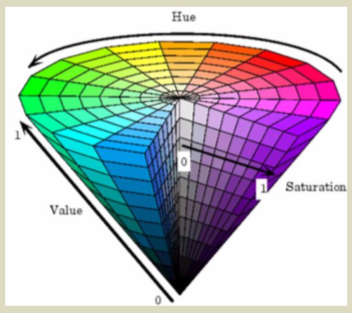
\includegraphics{colorwheel.png}
\caption{color wheel}
\end{figure}

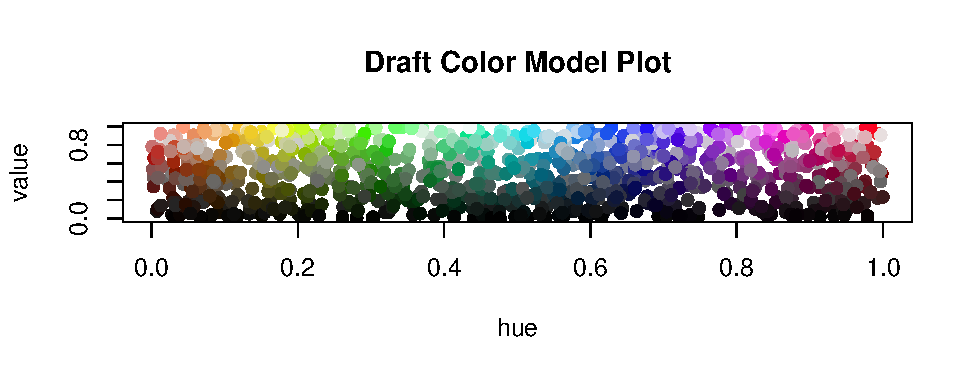
\includegraphics{design_files/figure-latex/unnamed-chunk-1-1.pdf}

\begin{Shaded}
\begin{Highlighting}[]
\FunctionTok{plot\_ly}\NormalTok{(}\AttributeTok{x =} \SpecialCharTok{\textasciitilde{}}\NormalTok{hue, }
        \AttributeTok{y =} \SpecialCharTok{\textasciitilde{}}\NormalTok{value, }
        \AttributeTok{z =} \SpecialCharTok{\textasciitilde{}}\NormalTok{saturation, }
        \AttributeTok{color =} \SpecialCharTok{\textasciitilde{}}\NormalTok{color)}
\end{Highlighting}
\end{Shaded}

\begin{quote}
R can use many different color models, but often uses a \#\textbf{R}ed,
\textbf{G}reen, \textbf{B}lue model with the amount of each color
indicated in Hexadecimal, 00 to FF, notation.
\end{quote}

\hypertarget{three-types-of-palettes}{%
\subsection{Three Types Of Palettes}\label{three-types-of-palettes}}

\url{http://colorbrewer2.org/}

\begin{Shaded}
\begin{Highlighting}[]
\FunctionTok{library}\NormalTok{(RColorBrewer)}
\end{Highlighting}
\end{Shaded}

\begin{Shaded}
\begin{Highlighting}[]
\FunctionTok{display.brewer.pal}\NormalTok{(}\DecValTok{7}\NormalTok{,}\StringTok{"Set1"}\NormalTok{) }\CommentTok{\# qualitative}
\end{Highlighting}
\end{Shaded}

\begin{figure}
\centering
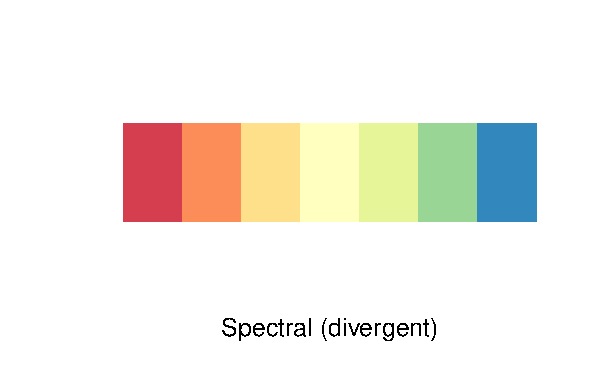
\includegraphics{design_files/figure-latex/unnamed-chunk-4-1.pdf}
\caption{Qualitative}
\end{figure}

\begin{Shaded}
\begin{Highlighting}[]
\FunctionTok{display.brewer.pal}\NormalTok{(}\DecValTok{7}\NormalTok{,}\StringTok{"YlOrRd"}\NormalTok{) }\CommentTok{\# sequential}
\end{Highlighting}
\end{Shaded}

\begin{figure}
\centering
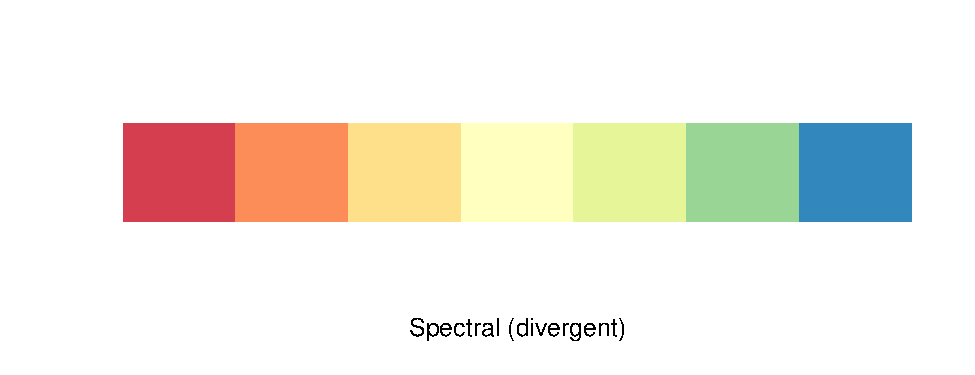
\includegraphics{design_files/figure-latex/unnamed-chunk-5-1.pdf}
\caption{Sequential}
\end{figure}

\begin{Shaded}
\begin{Highlighting}[]
\FunctionTok{display.brewer.pal}\NormalTok{(}\DecValTok{7}\NormalTok{,}\StringTok{"Spectral"}\NormalTok{) }\CommentTok{\# diverging}
\end{Highlighting}
\end{Shaded}

\begin{figure}
\centering

\includegraphics{design_files/figure-latex/unnamed-chunk-6-1.pdf}
\caption{Spectral}
\end{figure}

\begin{Shaded}
\begin{Highlighting}[]
\FunctionTok{display.brewer.all}\NormalTok{() }\CommentTok{\# all palettes}
\end{Highlighting}
\end{Shaded}

\begin{figure}
\centering
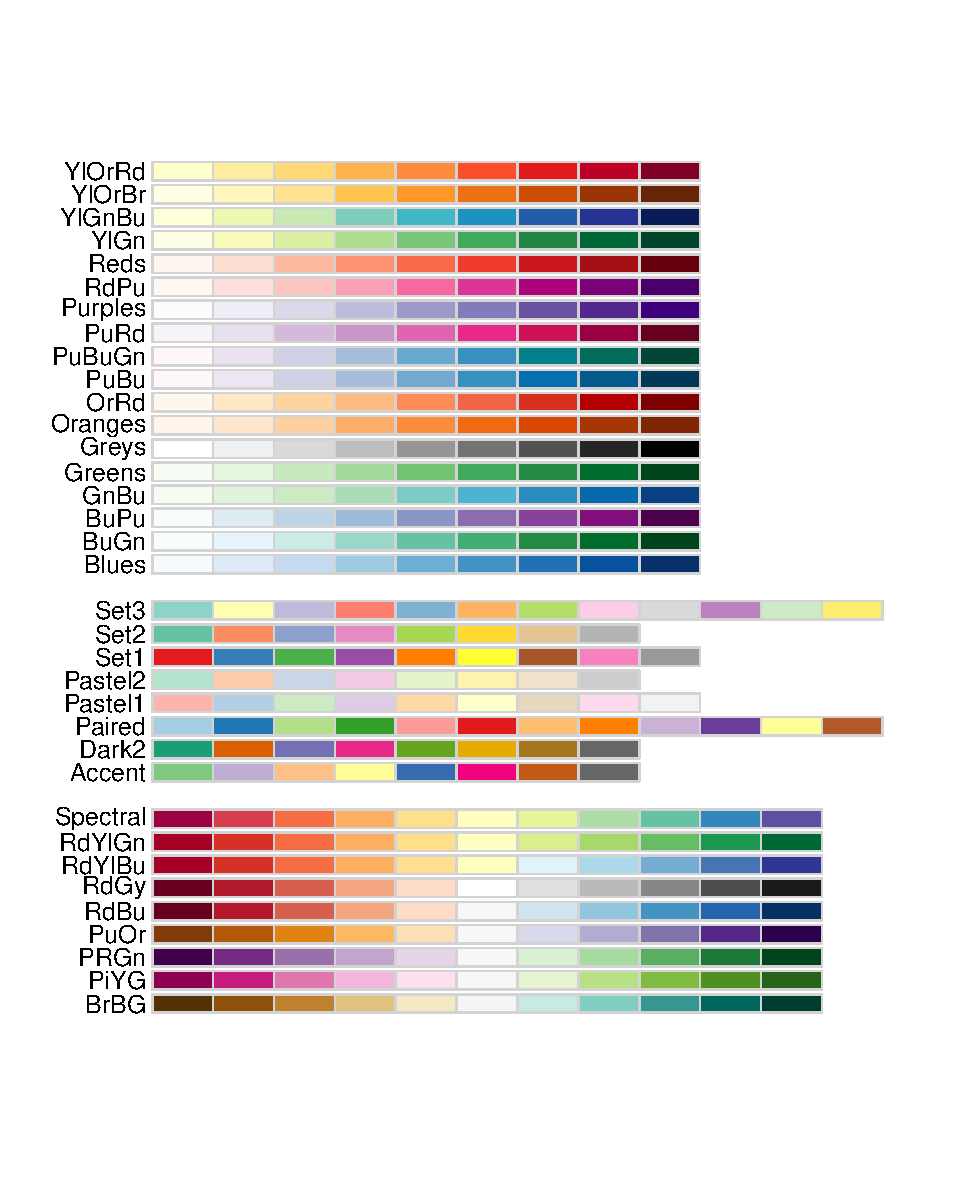
\includegraphics{design_files/figure-latex/unnamed-chunk-7-1.pdf}
\caption{All Palettes}
\end{figure}

\newpage

\hypertarget{where-do-the-colors-in-ggplot-come-from}{%
\subsection{\texorpdfstring{Where Do The Colors in \texttt{ggplot} Come
From?}{Where Do The Colors in ggplot Come From?}}\label{where-do-the-colors-in-ggplot-come-from}}

Equally spaced around the color wheel.

\begin{figure}
\centering
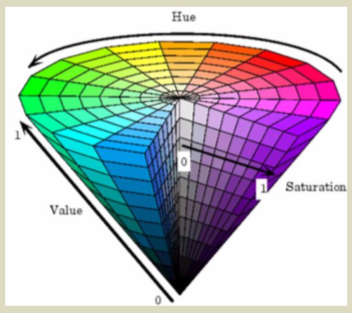
\includegraphics[width=0.2\textwidth,height=\textheight]{colorwheel.png}
\caption{color wheel}
\end{figure}

\begin{Shaded}
\begin{Highlighting}[]
\FunctionTok{library}\NormalTok{(scales)}

\FunctionTok{show\_col}\NormalTok{(}\FunctionTok{hue\_pal}\NormalTok{()(}\DecValTok{4}\NormalTok{))}
\end{Highlighting}
\end{Shaded}


\includegraphics{design_files/figure-latex/unnamed-chunk-8-1.pdf}

\hypertarget{color-is}{%
\subsection{Color is\ldots{}}\label{color-is}}

\begin{quote}
What is the purpose for which you are using color?
\end{quote}

\href{../political-social-work/index.html\#/color-scroll-down}{See these
notes} from my video lecture on Data Visualization in Political Social
Work.

\hypertarget{many-many-color-options}{%
\subsection{Many Many Color Options}\label{many-many-color-options}}

e.g.~Viridis, which is designed to be \emph{perceptually uniform}.

\begin{figure}
\centering
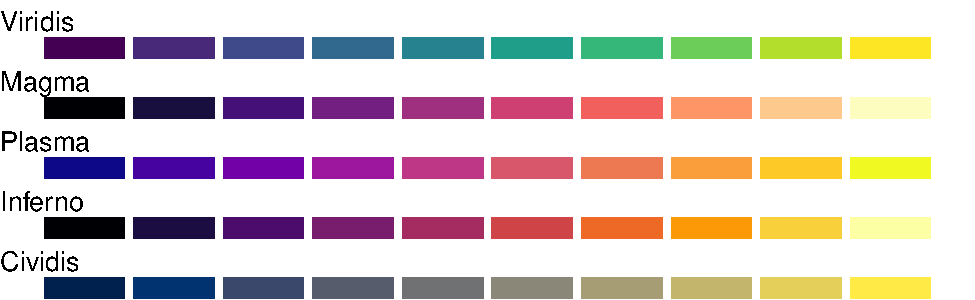
\includegraphics{design_files/figure-latex/unnamed-chunk-9-1.pdf}
\caption{Viridis Palettes}
\end{figure}

\hypertarget{other-color-and-palette-options}{%
\subsection{Other Color and Palette
Options}\label{other-color-and-palette-options}}

\begin{itemize}
\tightlist
\item
  \url{https://www.garrickadenbuie.com/project/ggpomological/}
\item
  \url{https://bbc.github.io/rcookbook/\#how_to_create_bbc_style_graphics}
\item
  \url{https://github.com/UI-Research/urbnthemes}
\end{itemize}

\hypertarget{fonts}{%
\section{Fonts}\label{fonts}}

\hypertarget{three-major-types-of-fonts}{%
\subsection{Three Major Types of
Fonts}\label{three-major-types-of-fonts}}

\begin{itemize}
\tightlist
\item
  San Serif e.g.~Arial, Helvetica
\item
  Serif Fonts e.g.~Times New Roman
\item
  \texttt{Monospaced\ Fonts} e.g.~\texttt{Courier} (good for code).
\end{itemize}

\hypertarget{font-rules}{%
\subsection{Font Rules}\label{font-rules}}

\hypertarget{dont-have-too-many-fonts}{%
\subsubsection{\texorpdfstring{Don't have \texttt{too\ many}
fonts!}{Don't have too many fonts!}}\label{dont-have-too-many-fonts}}

\hypertarget{interesting-font-for-heading-standard-font-for-text}{%
\subsubsection{Interesting Font For Heading; Standard Font For
Text}\label{interesting-font-for-heading-standard-font-for-text}}

\begin{quote}
Interesting Font for Heading
\end{quote}

\begin{quote}
Standard San Serif or Serif Fonts for text. Lorem ipsum dolor sit amet,
consectetur adipiscing elit, sed do eiusmod tempor incididunt ut labore
et dolore magna aliqua. Ut enim ad minim veniam, quis nostrud
exercitation ullamco laboris nisi ut aliquip ex ea commodo consequat.
Duis aute irure dolor in reprehenderit in voluptate velit esse cillum
dolore eu fugiat nulla pariatur. Excepteur sint occaecat cupidatat non
proident, sunt in culpa qui officia deserunt mollit anim id est laborum.
\end{quote}

\hypertarget{cognition}{%
\section{Cognition}\label{cognition}}

\hypertarget{dimensions-of-data}{%
\subsection{Dimensions of Data}\label{dimensions-of-data}}

\hypertarget{basic-idea-definition}{%
\subsubsection{Basic Idea / Definition}\label{basic-idea-definition}}

\begin{quote}
\emph{Dimensions} of the Data, \emph{Columns} of the Data,
\emph{Measures}, and \emph{Questions} are all terms essentially pointing
at the same concept.
\end{quote}

\begin{Shaded}
\begin{Highlighting}[]
\FunctionTok{data}\NormalTok{(iris) }\CommentTok{\# iris data set}

\FunctionTok{library}\NormalTok{(DT) }\CommentTok{\# nicely formatted data tables}

\FunctionTok{datatable}\NormalTok{(iris) }\CommentTok{\# dimensions of the data}
\end{Highlighting}
\end{Shaded}

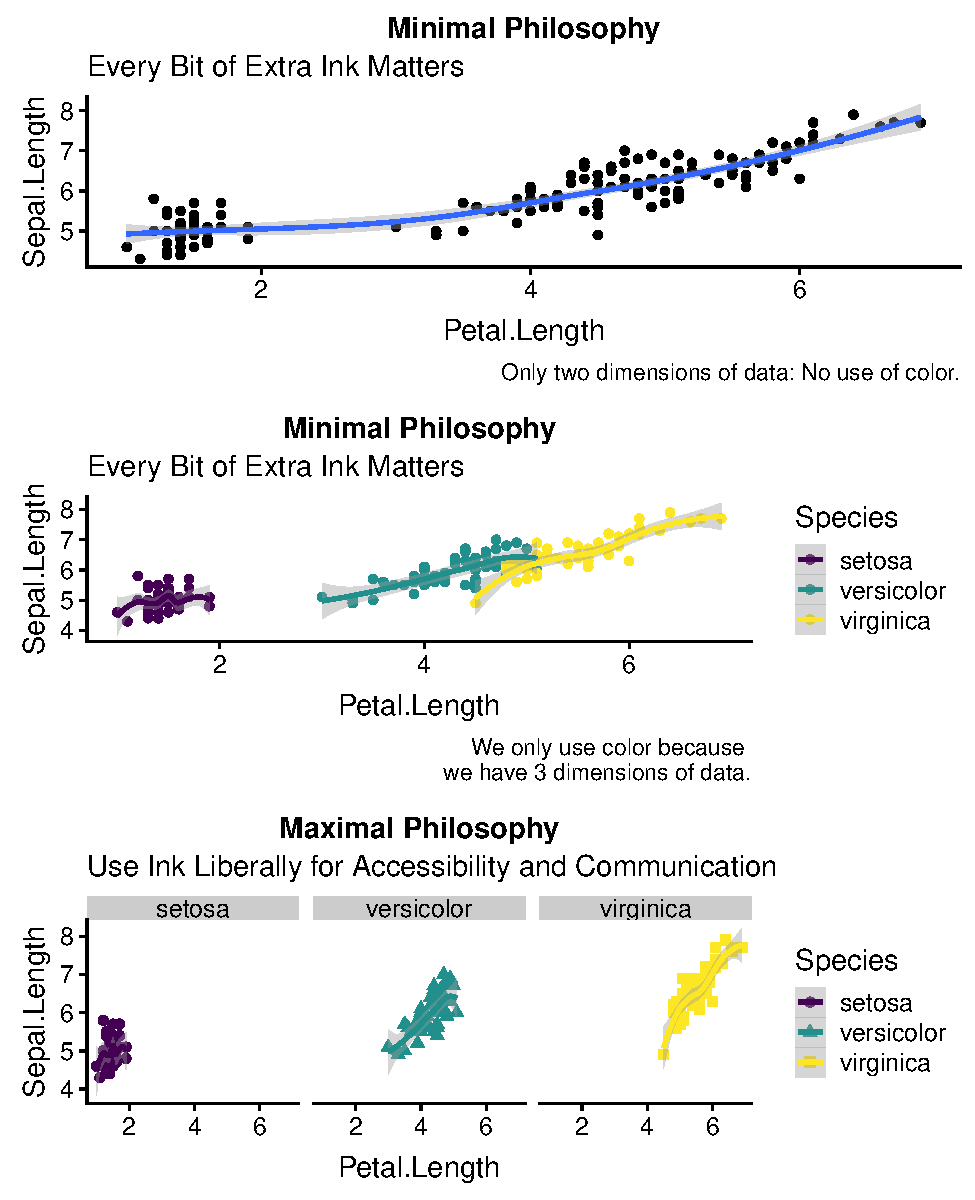
\includegraphics{design_files/figure-latex/unnamed-chunk-10-1.pdf}

\begin{quote}
The \texttt{iris} data set has 5 dimensions Sepal.Length, Sepal.Width,
Petal.Length, Petal.Width, Species.
\end{quote}

\hypertarget{species-of-iris}{%
\subsubsection{Species of Iris}\label{species-of-iris}}

Setosa:
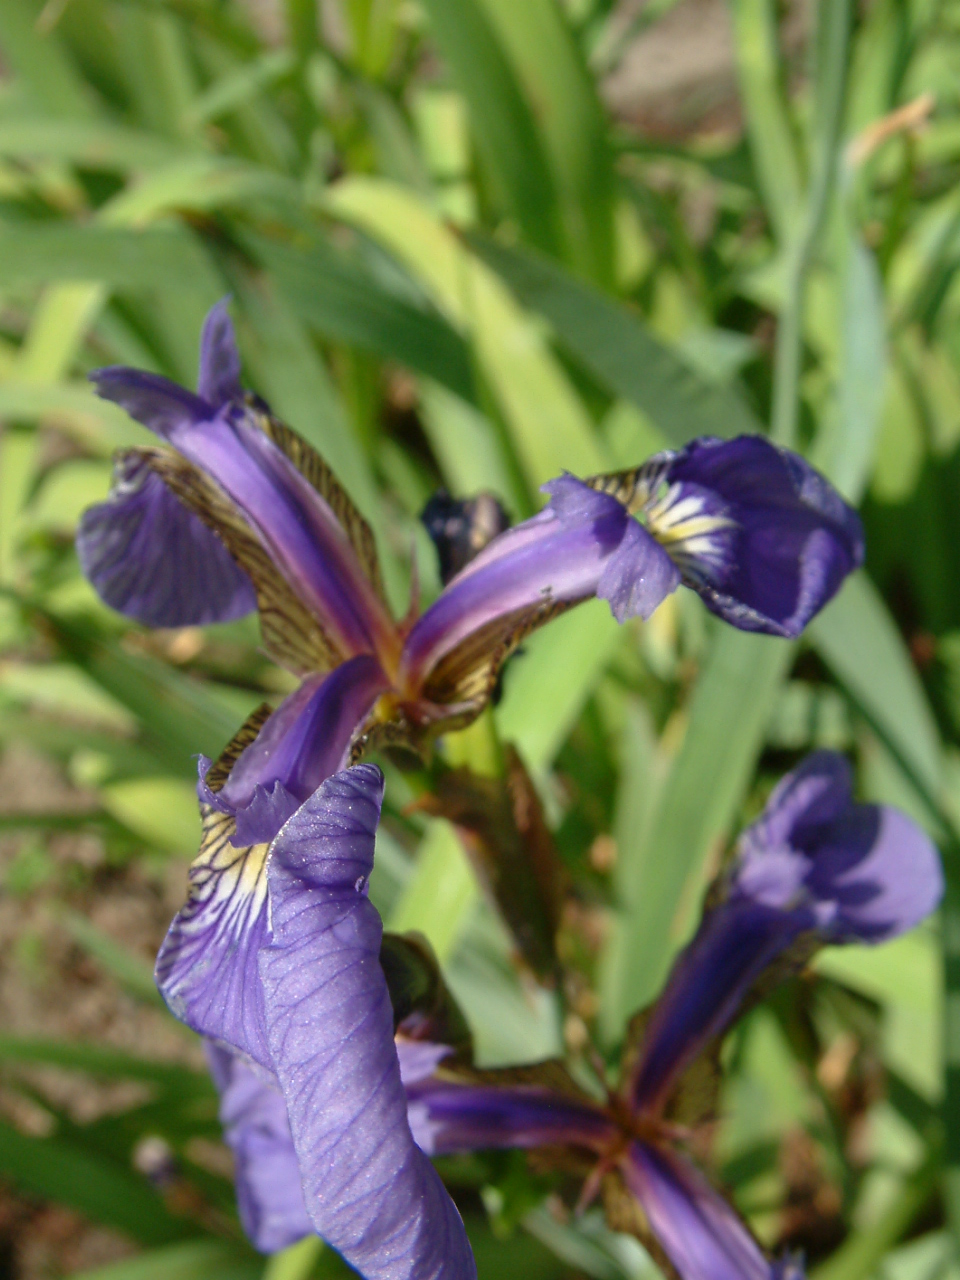
\includegraphics[width=0.2\textwidth,height=\textheight]{Kosaciec_szczecinkowaty_Iris_setosa.jpg}
Versicolor:
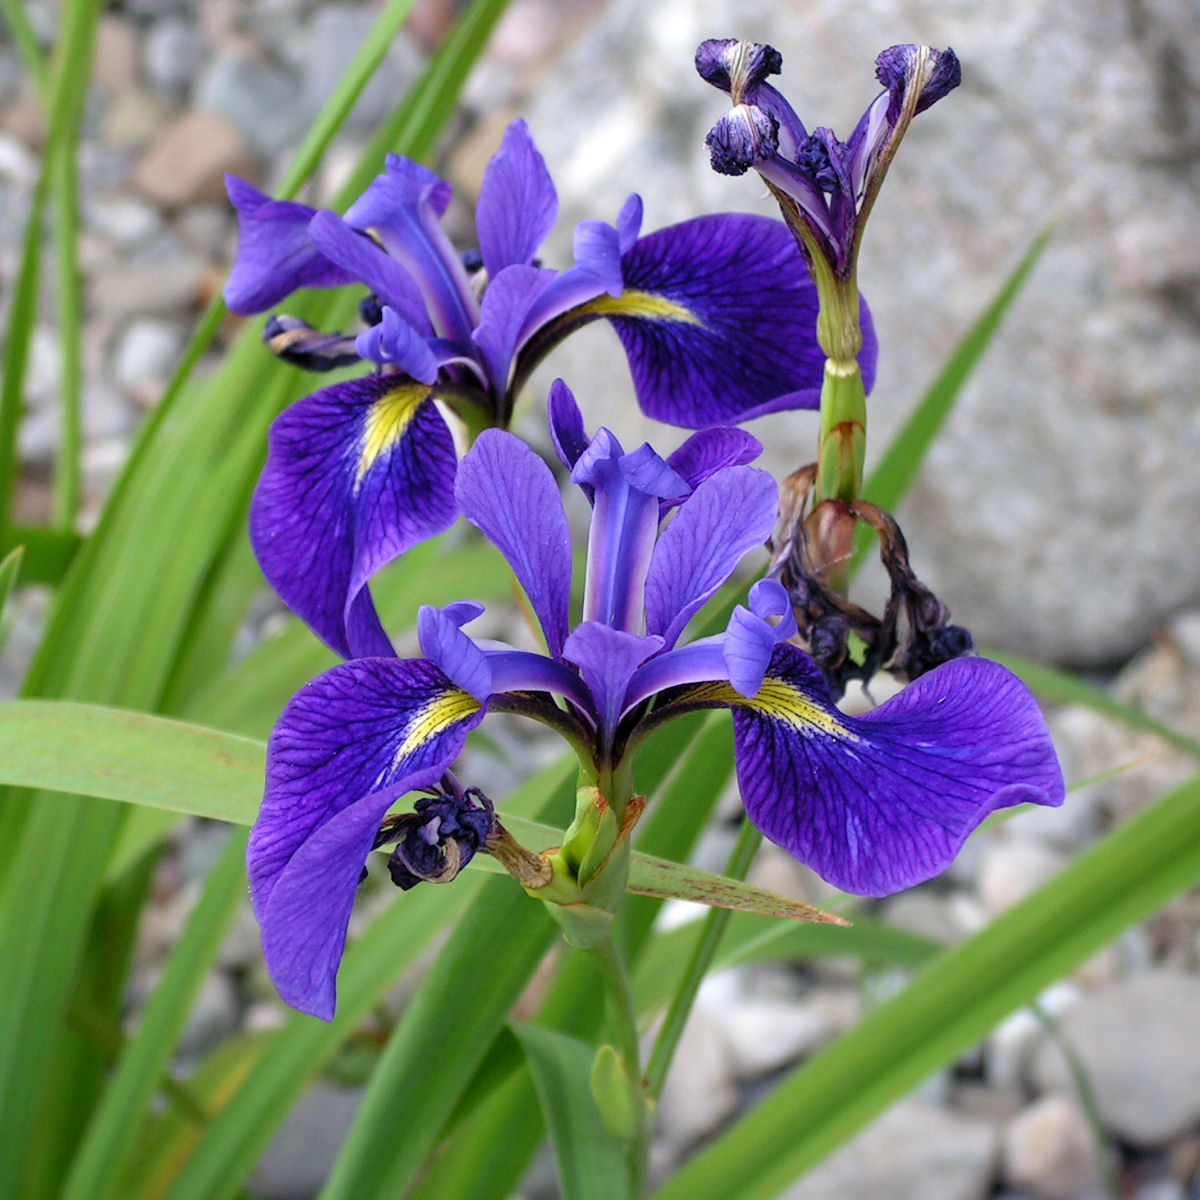
\includegraphics[width=0.2\textwidth,height=\textheight]{Blue_Flag_Ottawa.jpg}
Virginica:
\includegraphics[width=0.2\textwidth,height=\textheight]{Iris_virginica_2.jpg}

\begin{quote}
Iris species images courtesy
\href{https://www.wikipedia.org/}{Wikipedia}.
\end{quote}

\hypertarget{philosophies}{%
\subsubsection{Philosophies}\label{philosophies}}

\begin{figure}
\centering
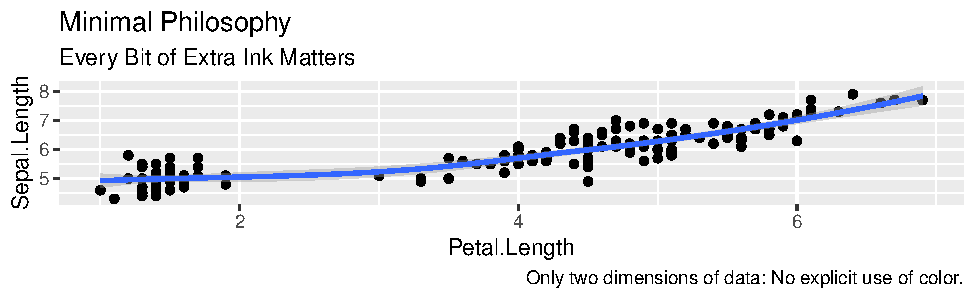
\includegraphics{design_files/figure-latex/unnamed-chunk-12-1.pdf}
\caption{Minimal Philosophy With 2 Data Dimensions}
\end{figure}

\begin{figure}
\centering
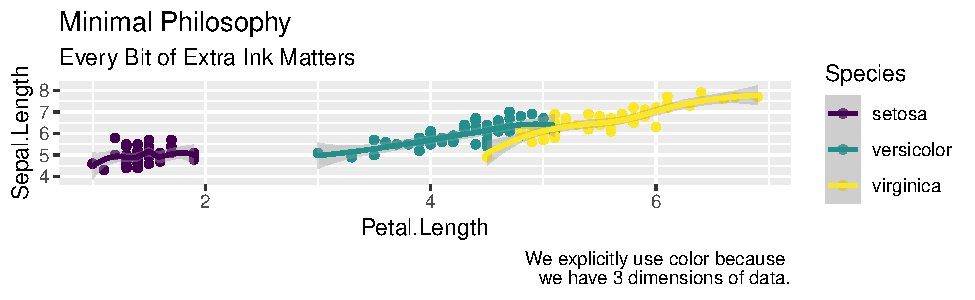
\includegraphics{design_files/figure-latex/unnamed-chunk-13-1.pdf}
\caption{Minimal Philosophy With 3 Data Dimensions}
\end{figure}

\begin{figure}
\centering
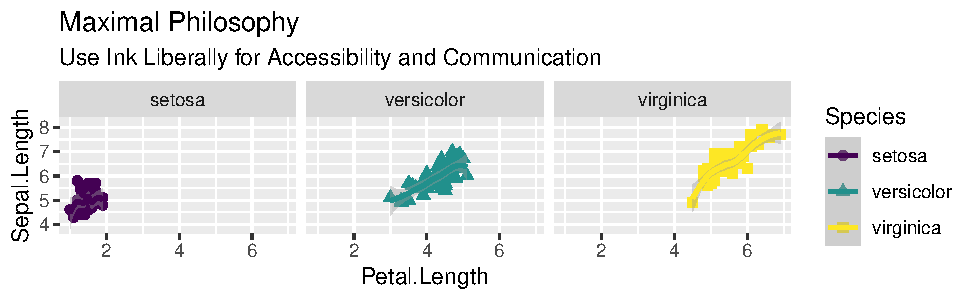
\includegraphics{design_files/figure-latex/unnamed-chunk-14-1.pdf}
\caption{Maximal Philosophy}
\end{figure}

\hypertarget{some-geometries-are-easier-to-understand-than-others}{%
\subsection{Some Geometries Are Easier To Understand Than
Others}\label{some-geometries-are-easier-to-understand-than-others}}

``Ordering elementary tasks by accuracy (Cleveland and McGill 1985):''

\begin{enumerate}
\def\labelenumi{\arabic{enumi}.}
\tightlist
\item
  Position along a common scale
\item
  Position on identical but nonaligned scales
\item
  Length
\item
  Angle \& Slope
\item
  Area
\item
  Volume, Density, Color Saturation
\item
  Color Hue
\end{enumerate}

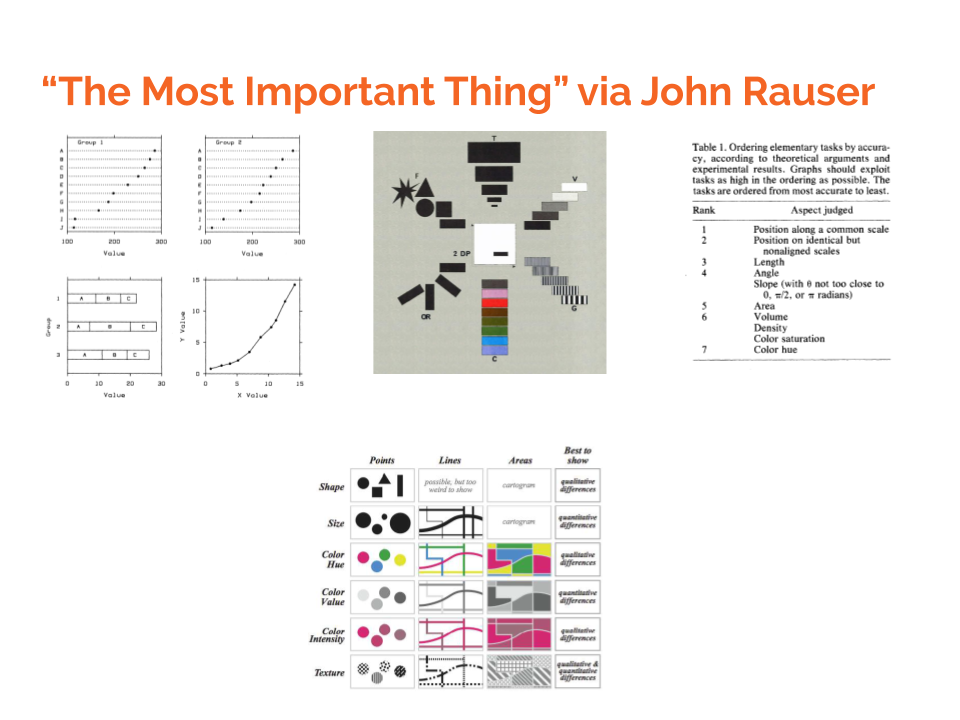
\includegraphics{Rauser-most-important-thing.png}

\hypertarget{references}{%
\section*{References}\label{references}}
\addcontentsline{toc}{section}{References}

\hypertarget{refs}{}
\begin{CSLReferences}{1}{0}
\leavevmode\vadjust pre{\hypertarget{ref-Cleveland1985}{}}%
Cleveland, William S, and Robert McGill. 1985. {``{Graphical Perception
and Graphical Methods for Analyzing Scientific Data}.''} \emph{Science}
229 (4716): 828--33. \url{http://www.jstor.org/stable/1695272}.

\end{CSLReferences}

\end{document}
